% !TeX program = pdflatex
% Unified rewrite, 2026-11-11. All numbers computed from master_unified_v1.csv
% (profile_v1 extraction) or from frozen model-layer verdicts (cited as such).
\documentclass[11pt,a4paper]{article}

\usepackage[T1]{fontenc}
\usepackage[utf8]{inputenc}
\usepackage{lmodern}
\usepackage[margin=2.4cm]{geometry}
\usepackage{amsmath,amssymb}
\usepackage{graphicx}
\usepackage{booktabs}
\usepackage{array}
\usepackage[colorlinks=true,linkcolor=blue,citecolor=blue,urlcolor=blue]{hyperref}
\usepackage{microtype}

\graphicspath{{figs/}}

\title{\bfseries Gating time constants are the conserved coordinates of cardiac
ion channels: a unified reanalysis of seven voltage-clamp corpora}

\author{Huan Li\\
\small Shanghai Liangta Biotech Co., Ltd.\\
\small \texttt{HL@liangtabio.com}}

\date{}

\begin{document}
\maketitle

\begin{abstract}
\noindent
Kinetic models of ion channels are written as rate-constant schemes, and the
schemes are known to be unidentifiable from voltage-clamp data. What the data
do identify has not been mapped at scale. We first show on a calibrated
thirteen-parameter hERG model that the identified subspace is seven-dimensional,
that the time scale is pinned by the waveform while amplitude is an exact gauge
direction, and that the identifiable content is therefore the set of modal
coordinates: time constants, steady-state curves and delays. We then measured
those coordinates directly. A single extraction pipeline, with per-row
profile-likelihood confidence intervals, was applied uniformly to seven public
voltage-clamp corpora, yielding a master table of 487,584 measured quantities
from 20,709 cells covering 74 channel types in seven families. The intervals
are calibrated (96.2\% coverage at the nominal 95\% level). On this table, one
pre-registered verdict separates the two kinds of quantity. Time constants are
conserved across cells while voltage midpoints drift: the midpoint scatter
exceeds the time-constant scatter in 63 of 64 activation groups (median ratio
2.47), in deactivation, inactivation and recovery groups, in all five HCN
groups with reversed gating polarity, in nine of ten layers of 933 published
models, and in 38 cross-species pairs where time constants stay within two-fold
while midpoints move by millivolts. Temperature separates the classes again:
activation carries the pooled $Q_{10}$ of 3.78 against 1.99 for deactivation,
and dividing 25\,$^\circ$C tables by pooled $Q_{10}$ values predicts 35\,$^\circ$C
kinetics with 94\% of 325 points inside a two-fold window. Across a
five-laboratory blinded hERG drug dataset reanalysed at waveform level, drugs
move occupancy and leave deactivation kinetics unchanged (median ratio 0.95,
flat against block depth, blinded cells reproducing the result). Models
assembled from the measured tables with one free conductance per cell predict
held-out CiPA drug-screening traces in 67 of 68 cells. Channel identity is
written in kinetics; cell state is written in midpoints.
\end{abstract}

\section{Introduction}

Kinetic models of cardiac ion channels are written as Hodgkin--Huxley or Markov
schemes and calibrated by global
optimisation~\cite{Colatsky2016,Li2017,Dutta2017,OHara2011,Clerx2016}.
The schemes differ in topology but share a parameterisation: one rate constant
per transition, chosen so that the model reproduces the recordings. The weakness
of that parameterisation is documented. In a survey of thirteen published Markov
models of cardiac channels, nine could not be determined uniquely from
step-clamp data, and the authors drew the consequence explicitly: where
parameters are unidentifiable, the layout of a model cannot be established from
the data, and the fitted values do not carry the mechanistic meaning usually
attributed to them~\cite{Fink2009}. The responses since have been richer
protocols~\cite{Beattie2018} and added constraints or
priors~\cite{Clerx2019}. Both leave the rate constants in place. What has not
been tested systematically is whether the data identify a different class of
quantity that can be measured directly and compared across cells, channels,
laboratories and species.

We reached the same conclusion by a different route. The question is not
academic. Cardiac safety pharmacology now runs on in silico models: the CiPA
initiative scores drug risk through channel models and a ventricular cell
model, and every regulatory submission inherits the identifiability problem
underneath~\cite{Colatsky2016,Dutta2017}. If the rate constants cannot be
recovered, a safety pipeline should rest on what can be recovered.

Our own hERG model was a
thirteen-parameter Markov-type scheme built from the published four-state ring
with a double-exponential activation edge and a parallel slow component. It
fitted the recordings and passed seven of eight pre-set criteria; it failed the
eighth on the sinusoidal protocol, after four rounds in which fixing the peak
broke the waveform and fixing the waveform broke the peak. Adding the states
that would repair the exclusion produced rate multipliers whose Cram\'er--Rao
bounds exceed the data window by a factor of about 760. The two failures are one
failure: expressiveness is bought with directions the data cannot see.

A Fisher analysis of the fitted model explains which directions those are, and
it points at what can be measured instead. We therefore rebuilt the analysis
from the measurement side. Seven public voltage-clamp corpora were re-extracted
from raw waveforms by one pipeline: local fits per protocol segment, no global
objective, and a profile-likelihood confidence interval on every extracted
quantity. The result is a single master table in which a hERG deactivation time
constant from a manual patch rig and a Kv1.1 activation time constant from a
high-throughput robot carry the same columns and the same uncertainty semantics.
On that table we ask four questions in sequence. Which quantities are shared
across cells? Does temperature move them? Do drugs move them? And do models
built from the shared quantities predict data they never saw?

The answer is consistent enough to state up front. Time constants are shared;
voltage midpoints are cell-specific. Temperature moves time constants by a
process-specific $Q_{10}$ and leaves midpoints flat. Drugs move occupancy and
leave kinetics essentially unchanged. And models assembled from measured tables
with a single free conductance per cell forward-predict held-out protocols,
held-out cells and held-out laboratories.

\section{Results}

\subsection{The identified coordinates are modal}

The starting point is a concrete failure. The thirteen-parameter hERG model
reproduces the four protocol families of its construction cell and passes seven
of eight pre-set criteria. The eighth fails informatively: the peak current and
the sinusoidal waveform cannot be satisfied by the same parameter set, the
exclusion persists across four re-parameterisation rounds, and the residual of
0.00096 in $R^{2}$ is an order of magnitude above run-to-run scatter while the
noise ceiling of the dataset sits at $R^{2}\ge0.973$. The residual is model
error, not benchmark artefact. Adding serial closed states repairs the waveform
and forfeits the parameters: the repaired variant passes all eight criteria,
but its rate multipliers carry Cram\'er--Rao bounds of $\pm9.6$--$13.2$\,dex
against a data window of $\pm0.017$\,dex.

The Fisher information of the calibrated thirteen-parameter hERG model,
\begin{equation}
F_{ij} = \frac{1}{\sigma^{2}}\sum_{t}
\frac{\partial I(t;\boldsymbol{\theta})}{\partial\theta_i}\,
\frac{\partial I(t;\boldsymbol{\theta})}{\partial\theta_j},
\label{eq:fisher}
\end{equation}
was evaluated by central finite differences on an independent simulation channel
with per-segment residual variance as weights. The thirteen eigenvalues span
12.9 orders of magnitude. Six directions sit below $10^{-3}$ of the largest, so
the data identify a seven-dimensional subspace of the thirteen-dimensional
parameter space. The null space is structured. One degeneracy is exact: with the
maximum open probability frozen, the combination
$\alpha_{\mathrm{amp}}\cdot\mathrm{ALPHA}\cdot\mathrm{XMAX}$ enters only as a
product, and no experiment can separate its factors. One is near-exact: the two
exponential components of the activation edge can be exchanged at a cost
consistent with machine precision
($\lambda/\lambda_{\max}\approx1.4\times10^{-13}$).

The degeneracy usually assumed in this literature is not there. A joint
rescaling of all rate constants by $s$ with the conductance by $1/s$ is often
treated as leaving voltage-clamp protocols invariant; it does not. On a fixed
protocol time grid,
\begin{equation}
I_s(V,t) = \frac{1}{s}\,I(V,st) \neq I(V,t),
\label{eq:rescale}
\end{equation}
and a 10\% rescaling changes the predicted waveform by 18--45\%, far outside the
noise. The data pin the time scale. What they do not pin is the amplitude scale:
because the current factorises as
\begin{equation}
I(t) = g\,\Phi(t;\boldsymbol{\theta}),
\label{eq:factor}
\end{equation}
with $g$ the conductance and $\Phi$ the shape, the Fisher information about the
shape parameters obeys $F_{\boldsymbol{\theta}\boldsymbol{\theta}} = g^{2}F_{0}$,
independent of $g$. The shape subspace and the scale direction decouple exactly.
Amplitude is a gauge direction; time is not. The identified coordinates of a
gating model are therefore the modal ones: how fast the current rises and falls
at each voltage, where it sits at steady state, how long opening is delayed.
These are observables of protocol-rich recordings, not fitting targets.

\subsection{One measurement pipeline over seven corpora}

We applied one extraction pipeline uniformly to seven public voltage-clamp
corpora (Table~\ref{tab:data}): the Channelpedia automated-patch collection
(17,987 cells after quality control, 66 Kv-family channel types plus HCN, Kir,
K2P and other families), the five-laboratory blinded hERG drug dataset
coordinated by HESI under the FDA Broad Agency Announcement (28 drugs, 1,875
cells passing trace-level quality control), the five-temperature hERG series of
Lei and colleagues (670 wells), the nine-cell manual hERG dataset of Beattie and
colleagues, a Nav1.5 whole-cell series at two temperatures, a Ca\textsubscript{v}1.2
series with continuous bath-temperature readout, and an I\textsubscript{Ks}
activation series (283 recordings). Every protocol segment was reduced locally:
mono- or bi-exponential fits to activation, inactivation, deactivation and tail
segments; Boltzmann fits to steady-state curves; delays by back-extrapolation.
No objective function couples protocols or parameters at any stage.

The corpora differ in structure, and the pipeline meets each on its own terms.
For the CiPA dataset the sweep metadata exist for only one laboratory, so
vehicle, drug-block and steady-state windows were segmented from the waveform
plateaus alone, voltage-contaminated current columns in three laboratories were
detected and excluded, and current units were read from column suffixes (the
two official numerical disasters and the unit pitfalls found in the public
tables are listed in the Supplementary Information). For the nine-cell manual
dataset, steady-state activation was measured by the tail-current method rather
than the holding-segment mean, which removes a Boltzmann degeneracy that would
otherwise push the midpoint fits to their bounds. For Nav1.5 the inactivation
time constant was measured from peak-aligned decay windows at 40\,µs sampling.
For Ca\textsubscript{v}1.2 the bath-temperature channel was carried alongside
each sweep, so temperature enters as a measured covariate rather than a nominal
label. For I\textsubscript{Ks} the activation delay and time constant were fit
jointly on the step epoch and the deactivation time constant on the $-40$\,mV
tail epoch, with duplicate recordings of the same cell resolved to a single
best version before fitting.

Each extracted quantity carries a per-row profile-likelihood 95\% confidence
interval rather than a symmetric standard error. The intervals matter for two
reasons. They are honest where the likelihood is asymmetric (the median upper to
lower half-width ratio across the Channelpedia corpus is 1.43, so symmetric
errors systematically understate the upward uncertainty), and they are
calibrated: across the 255,411 quality-passed time-constant rows of the master
table, the nominal 95\% intervals contain the point estimate at 96.2\%, with
per-source coverage between 93.4\% and 100\% (Fig.~\ref{fig:corpus}c). Rows whose
fit touches a window boundary are flagged rather than deleted (for example the
Ba$^{2+}$-carried Ca\textsubscript{v}1.2 records, where inactivation is too slow
for the 180\,ms window), and they enter every statistic with their flag.

The merged table holds 487,584 measured quantities from 20,709 cells across 74
channel types in seven families, with source, cell, protocol, value, interval,
quality flag and method version on every row (Fig.~\ref{fig:corpus}a,b). Three
reference layers are stored in the same schema: the official CiPA potency anchors
for 29 drugs across seven channels, 38 cross-species group comparisons, and ten
gating-layer summaries of 933 published models from the ICGenealogy model
library, refit in-house. All analysis below reads this table and nothing else.

\begin{figure}[htbp]
\centering
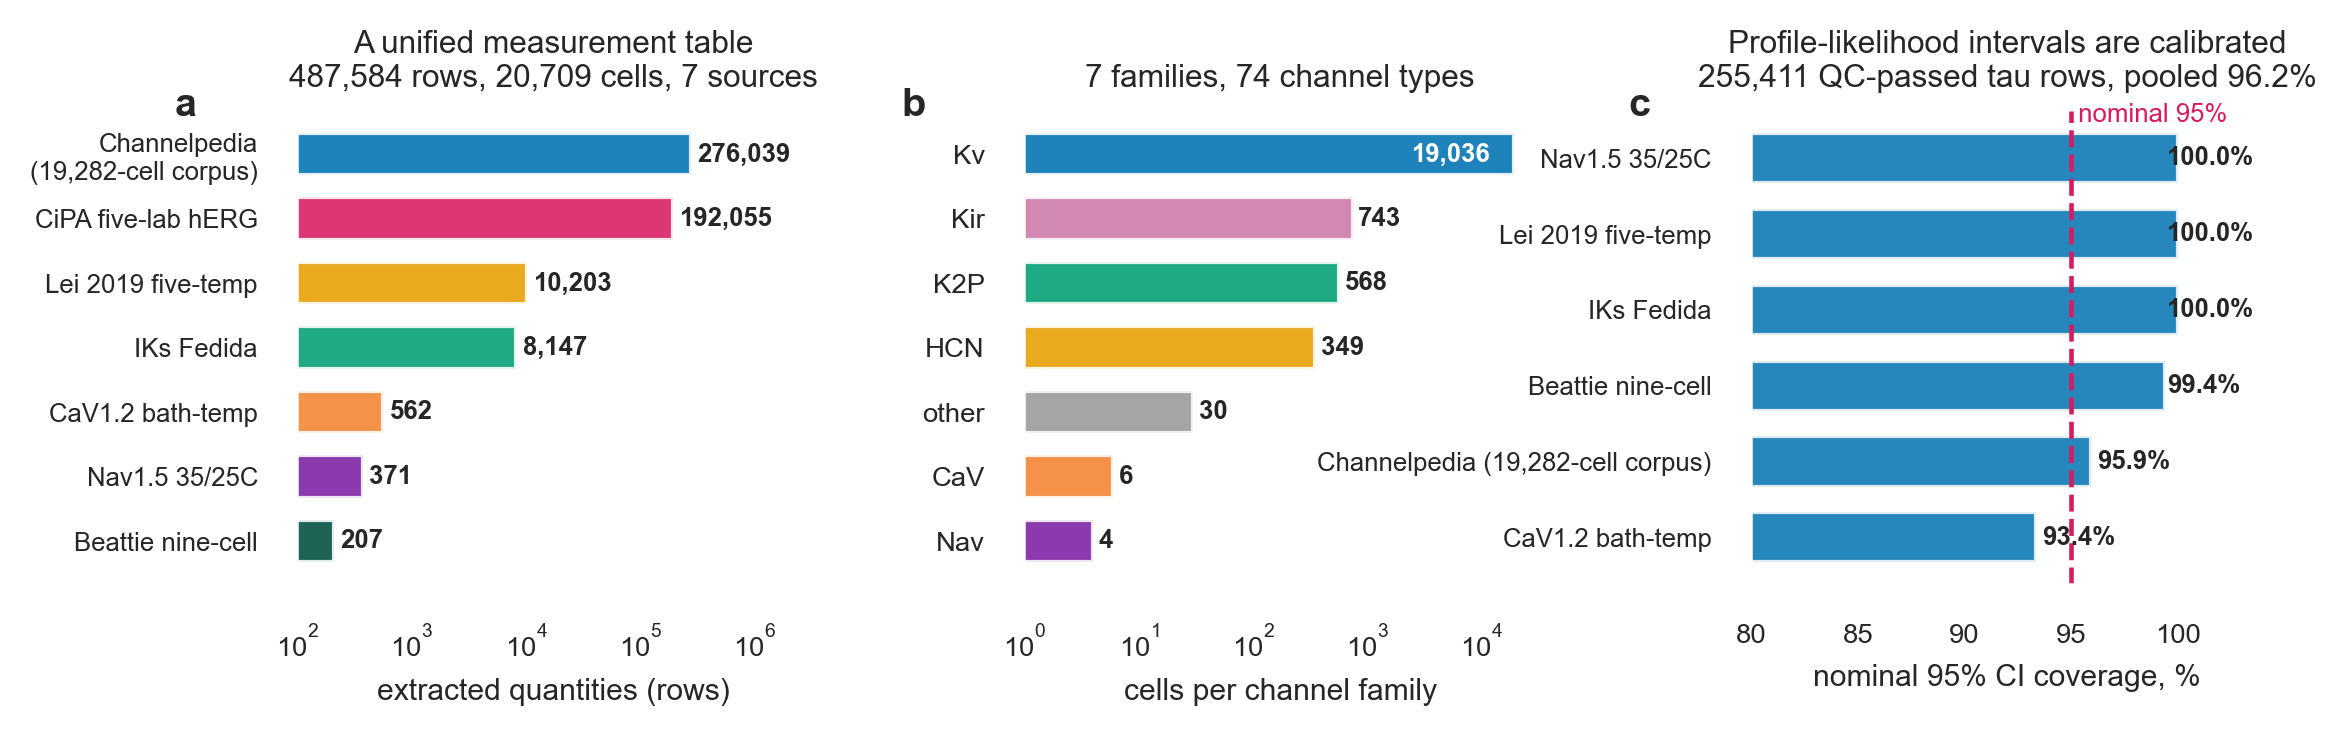
\includegraphics[width=\linewidth]{fig1_method_corpus.png}
\caption{\textbf{One extraction pipeline, one table.} (a) Measured quantities
per corpus (rows of the master table). (b) Cells per channel family.
(c) Calibration of the per-row profile-likelihood intervals: coverage of the
point estimate by the nominal 95\% interval, per corpus (quality-passed
time-constant rows only; pooled coverage 96.2\%, $n=255{,}411$).}
\label{fig:corpus}
\end{figure}

\subsection{Time constants are conserved, midpoints are not}

For every group of cells of one channel type at one temperature we computed two
scatters: the scatter of the time constant across cells at fixed voltage, in
dex, and the scatter of the steady-state midpoint across cells, in units of the
Boltzmann slope $k$ (so that both are dimensionless measures of relative
dispersion). The verdict rule is the ratio of the two, with group-level shrinkage
by hierarchical partial pooling and per-row uncertainties propagated from the
profile intervals. A ratio above one means the time constant is the more
conserved quantity.

The verdict is nearly unanimous, and it is the same verdict at every level of
organisation (Fig.~\ref{fig:law}a). In the Channelpedia corpus the main
activation judgement passes in 63 of 64 pure-Kv groups (98.4\%), with median
ratio 2.47. The same rule holds for deactivation (43 of 48, median 2.82),
inactivation (28 of 35, median 1.33) and recovery from inactivation (39 of 42,
median 2.15). The HCN family, whose gating polarity is reversed, passes all five
of its groups with median ratio 8.03, and its subtype midpoint ordering
(HCN1 $>$ HCN2 $>$ HCN4 $>$ HCN3) reproduces the literature, a lateral check that
the extractor reads both directions of gating correctly. The rule also holds in
the published-model layer: across 933 deduplicated models from ICGenealogy,
whose gating curves we refit individually, nine of ten family-by-gate layers pass
(median 2.07), the exception being the small and highly inbred I\textsubscript{H}
model set, which ties at 1.00. Finally, between species, the time constant stays
within two-fold in 38 of 38 cross-species channel pairs while midpoints differ by
up to tens of millivolts (Fig.~\ref{fig:law}c).

The single failure of the main verdict is registered rather than smoothed over.
Kv3.2 at 15\,$^\circ$C returns a ratio of 0.83: its kinetic scatter is among the
largest in the corpus and its midpoint scatter the smallest, so this channel at
this temperature stores its diversity in kinetics, as its source study also
notes. We also tested the window-current hypothesis, that activation and
inactivation midpoints of one cell are jointly constrained; it is negative
(median correlation 0.30 across 35 channel-temperature pairs), so the two
midpoints are independent set points of the cell.

The verdict is stable under four changes of calibre. Removing the Boltzmann
fits that hit their voltage bounds leaves 63 of 64 groups passing (median
2.87). Replacing the two-stage variance decomposition by full hierarchical
partial pooling shrinks both sides and leaves the verdict unchanged (63 of 64,
median 2.48). Replacing symmetric standard errors by the profile-likelihood
intervals changes exactly one of the 194 group verdicts across the five tables
(Kv1.7 at 15\,$^\circ$C moves from 1.009 to 0.995, sitting on the threshold in
both calibres) and leaves the main verdict at 63 of 64 with median 2.47. And
the hierarchical time-constant estimates differ from the frozen values by a
median of $-1.3\%$ per group, so the scatter estimates are nearly unbiased.
The 66-group frame of earlier drafts contained two TASK-3 groups; K2P leak
channels have no sigmoidal gating and were registered as a grouping impurity,
giving the 64-group frame used here.

Fig.~\ref{fig:law}b shows the raw geometry behind one verdict group. In Kv1.1 at
25\,$^\circ$C the activation time constant at fixed voltage clusters within 0.58
dex across 592 cells, while the activation midpoint spreads over 8.65 slope units.
The conservation statement is therefore not about measurement precision but about
what is variable between cells: the cell sets its operating point, and it
inherits its kinetics.

\begin{figure}[htbp]
\centering
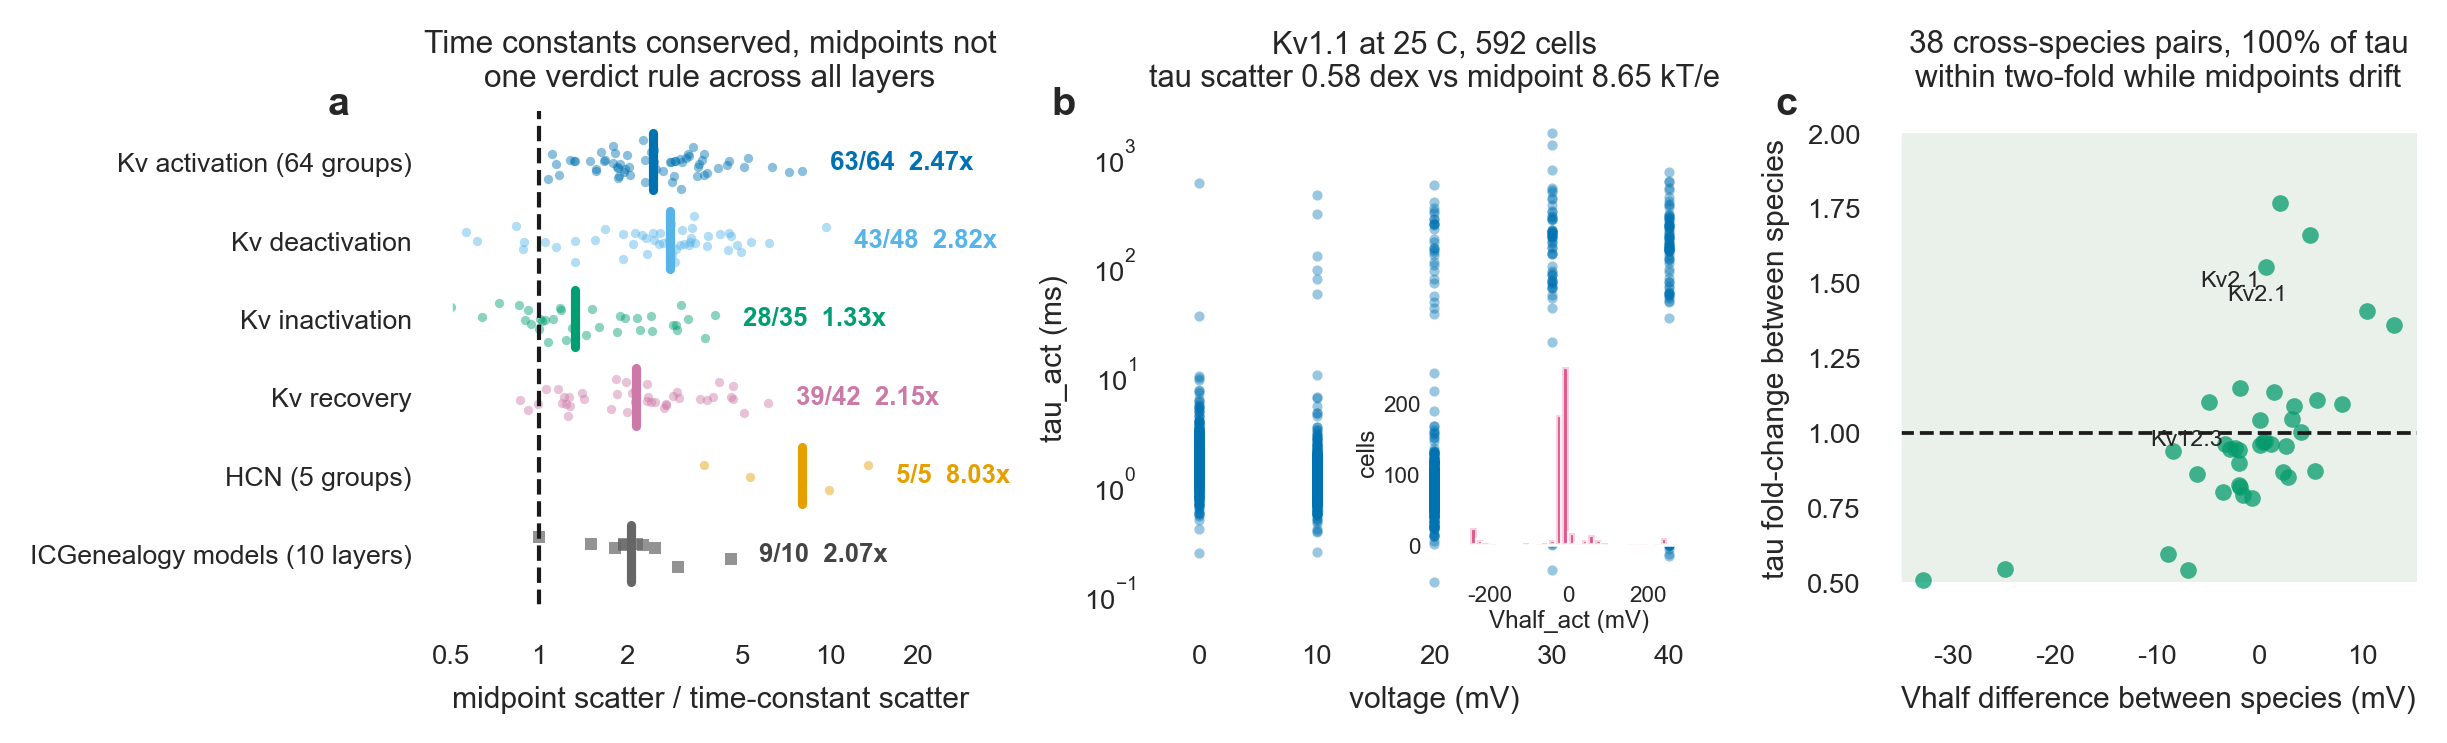
\includegraphics[width=\linewidth]{fig2_law_panorama.png}
\caption{\textbf{One verdict rule across all layers.} (a) Ratio of midpoint
scatter to time-constant scatter per group, for five experimental layers and the
published-model layer; points are groups, bars are medians, and the dashed line
marks equality. Counts and medians use the shrunk (partial-pooling) estimates
with profile-interval uncertainties. (b) One group in raw form: Kv1.1 activation
time constants at 25\,$^\circ$C versus voltage across 592 cells; inset, the
midpoint distribution of the same cells. (c) Cross-species pairs: time-constant
fold-change against midpoint difference for 38 pairs; the band marks two-fold.}
\label{fig:law}
\end{figure}

\subsection{Temperature separates the two classes and carries a forecast}

If kinetics are channel identity and midpoints are cell state, temperature should
move the first in an organised way and need not move the second at all. That is
what the table shows. In the five-temperature hERG series (670 wells,
25--37\,$^\circ$C), the recovery time constant follows $Q_{10}=2.91$, the fast
activation component 2.37 and the fast deactivation component 2.79, each monotone
across the five temperatures (Fig.~\ref{fig:temp}a). In the Channelpedia corpus,
where many channel types were recorded at more than one temperature, the pooled
$Q_{10}$ is 3.78 for activation ($n=202$ channel-process pairs), 1.99 for
deactivation ($n=74$) and 1.84 for inactivation ($n=65$): temperature loads on
activation across the family (Fig.~\ref{fig:temp}b). Midpoints, in contrast, are
flat in temperature at the family level (median $-0.05$\,mV per $^\circ$C); the
two bidirectional midpoint drifts reported for
hERG~\cite{Vandenberg2006,Li2016} are hERG-specific, not a general rule.

The Ca\textsubscript{v}1.2 corpus adds a continuous readout: bath temperature was
recorded on a third channel during pharmacology ramps, and the calcium-dependent
inactivation time constant, extracted per sweep, decreases gently with
temperature (apparent $Q_{10}\approx1.4$ over 32--38.5\,$^\circ$C;
Fig.~\ref{fig:temp}d), consistent with a process carried more by calcium binding
than by a protein conformational change.

Temperature then gives the strongest test available to a measurement table: a
zero-parameter forecast. Dividing the 25\,$^\circ$C population time-constant
tables by the pooled per-channel, per-process, per-voltage $Q_{10}$ predicts the
35\,$^\circ$C population tables with no free parameter. Of 325 predicted points
across 20 channel types, 94\% land within a two-fold window of the measured 35
$^\circ$C values and the median fold error is 28\% (Fig.~\ref{fig:temp}c). The
prediction errors are not random: they concentrate where the 25\,$^\circ$C
population is thin, which is a sampling limit rather than a method limit.

\begin{figure}[htbp]
\centering
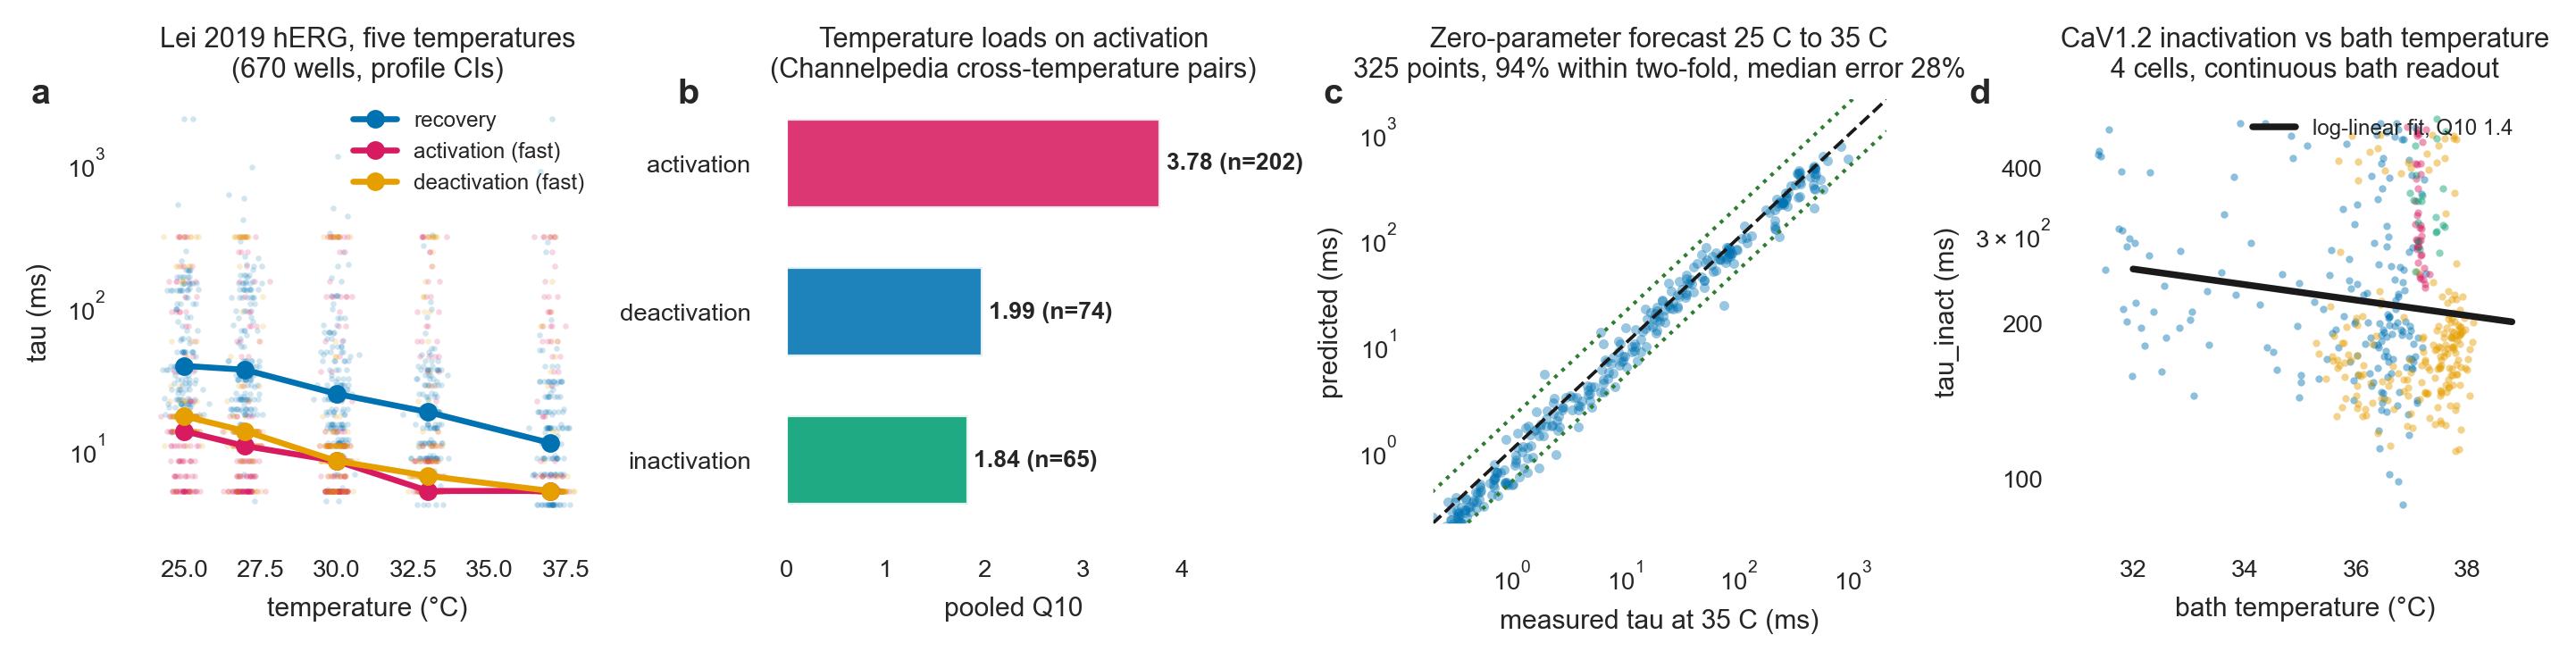
\includegraphics[width=\linewidth]{fig3_temperature.png}
\caption{\textbf{Temperature moves kinetics, not midpoints.} (a) The
five-temperature hERG series: per-well time constants (light points) and medians
(lines) for three processes. (b) Pooled $Q_{10}$ by process across the
Channelpedia cross-temperature pairs. (c) Zero-parameter forecast of 35\,$^\circ$C
kinetics from 25\,$^\circ$C tables divided by pooled $Q_{10}$; dotted lines mark
the two-fold window. (d) Ca\textsubscript{v}1.2 inactivation time constant against
continuously recorded bath temperature, with the log-linear fit.}
\label{fig:temp}
\end{figure}

\subsection{Drugs move occupancy, not kinetics}

We reanalysed the five-laboratory blinded hERG dataset at waveform level with the
same profile pipeline (1,750 cells contributing deactivation windows, 192,055
extracted sweep-level quantities).
For each cell the deactivation time constant of tail currents under drug was
referenced to the vehicle segment of the same cell, with the steady-state
(highest-concentration) block as the test window. Across 970 cells with both
segments valid, the median ratio of drug to vehicle time constant is 0.948
(Fig.~\ref{fig:drug}a). The ratio does not drift with block depth: binned by
steady-state block fraction, the stratum medians run 0.96, 0.90, 0.89, 1.01 and
1.07 from shallow to deep block (Fig.~\ref{fig:drug}b), so whatever small kinetic
modulation exists is bounded, does not scale with occupancy, and no drug doubles
or halves the time constant. Per-laboratory medians are 1.05, 0.99, 0.81, 0.92
and 1.17; the laboratory-3 value corresponds to a 19\% acceleration and is the
largest deviation in the dataset. The blinded arm reproduces the unblinded one
through the same frozen pipeline (medians 0.87 against 0.96;
Fig.~\ref{fig:drug}c), which is the internal control against analyser bias.
Potency anchors are reproduced independently: our per-drug IC$_{50}$ estimates
match the official CiPA values within ten-fold for 23 of 24 drugs
(Fig.~\ref{fig:drug}d).

Occupancy itself is not simple one-to-one pore plugging. Three waveform-level
signatures indicate state-dependent binding: Hill coefficients differ from one in
42 of 134 drug-laboratory sets; in deep block the residual current has a
different shape ratio than simple scaling predicts (0.73 in laboratory 1); and
the onset of block does not plateau within either exposure in 36--39\% of cells.
The apparent on-rate is not measurable in this dataset at all: it is flattened by
solution exchange (log-log slope against concentration approximately zero), so
this dataset pins equilibrium quantities and not binding kinetics, a limitation
we register explicitly.

The same invariance appears outside hERG. In the Nav1.5 two-temperature series,
the inactivation time constant at 35\,$^\circ$C is flat across the five
compound levels of that study (medians 0.25--0.36\,ms; Fig.~\ref{fig:cards}a,
inset), so the drug-independence of kinetics is not an hERG peculiarity.

\begin{figure}[htbp]
\centering
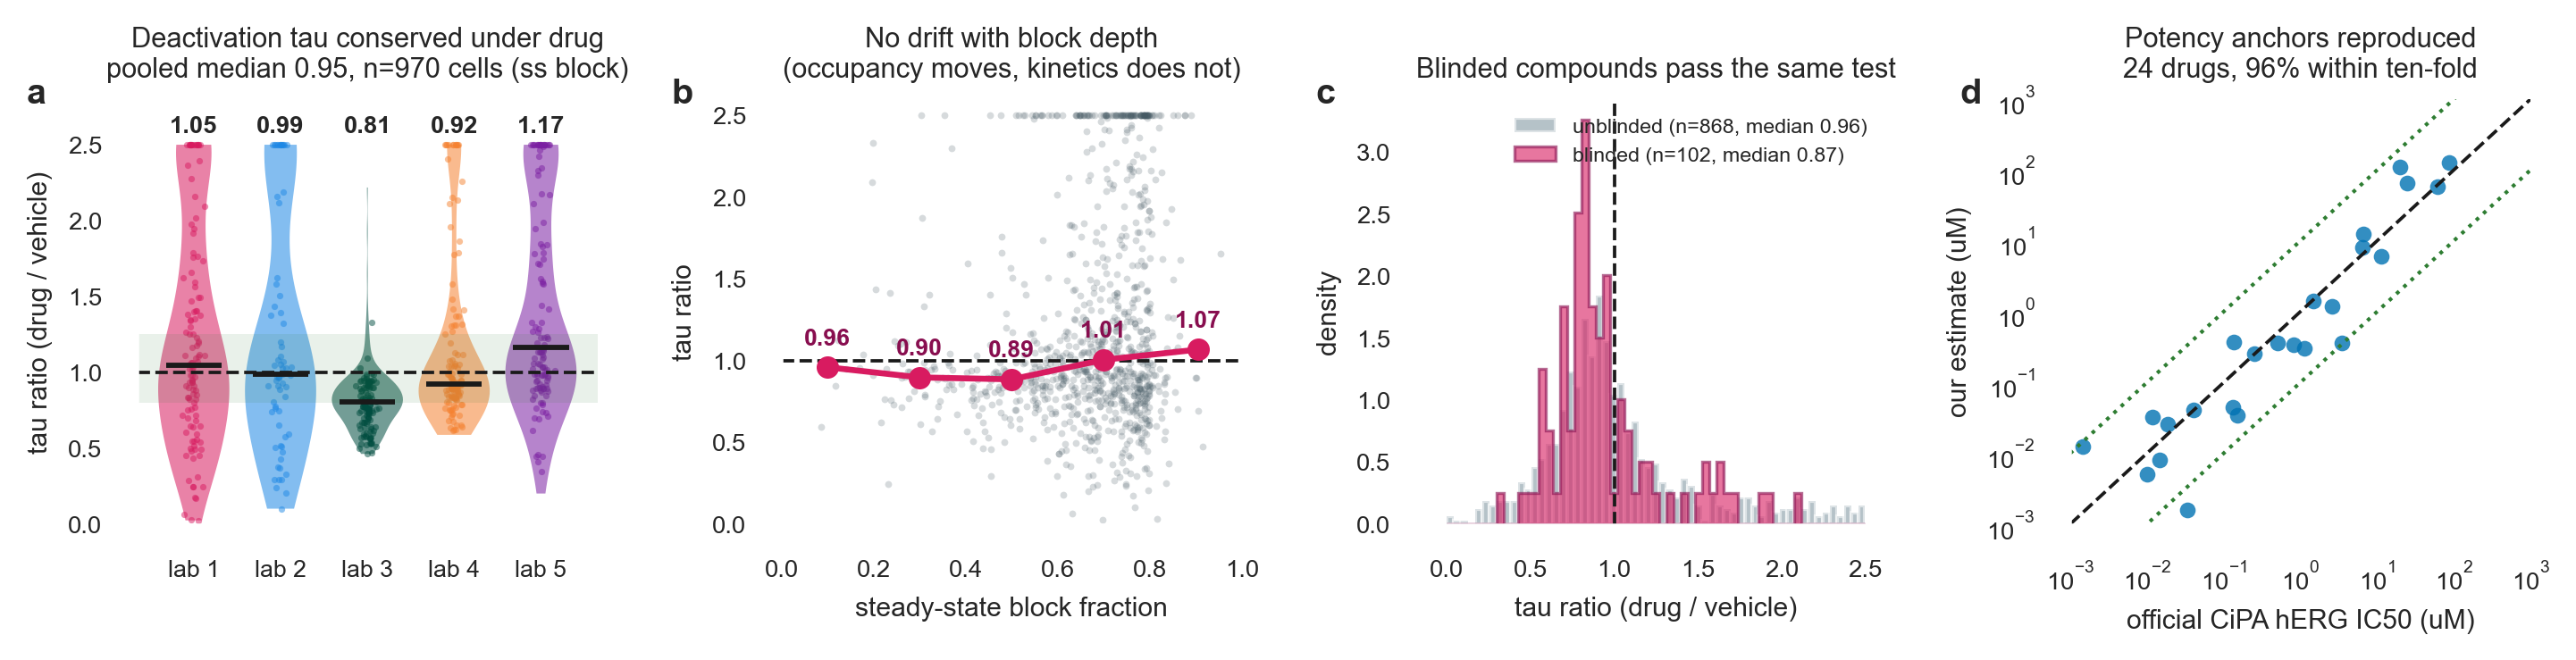
\includegraphics[width=\linewidth]{fig4_drug.png}
\caption{\textbf{Drugs move occupancy, not kinetics.} (a) Deactivation
time-constant ratio, drug versus vehicle within cell, per laboratory (violins;
medians marked; green band 0.80--1.25; steady-state block window).
(b) The same ratio against steady-state block fraction, with stratum medians.
(c) Blinded and unblinded cells through the same frozen pipeline. (d) Potency
anchors: our per-drug IC$_{50}$ estimates against the official CiPA values;
dotted lines mark ten-fold.}
\label{fig:drug}
\end{figure}

\subsection{The channel cards}

The remaining three corpora extend the same picture beyond the Kv family
(Fig.~\ref{fig:cards}). Nav1.5 inactivation kinetics are fast and tight: at
35\,$^\circ$C the inactivation time constant runs from 0.22 to 0.37\,ms across
the voltage range, four cells agreeing within a narrow band, and the 25\,$^\circ$C
series sits systematically slower as the temperature law requires
(Fig.~\ref{fig:cards}a). Ca\textsubscript{v}1.2 calcium-dependent inactivation at
+47\,mV has a median time constant of 195\,ms across six cells with the fit
ceiling registered where the carrier is Ba$^{2+}$ (Fig.~\ref{fig:cards}b).
I\textsubscript{Ks} is the slow counterpart of hERG: activation time constants
form the characteristic bell between 0.2 and 0.6\,s and deactivation sits near
450\,ms across 283 recordings, with the interquartile band narrow at every
voltage (Fig.~\ref{fig:cards}c). In the nine manual hERG cells the deactivation
ladder is reproduced cell by cell (slow component 3.6\,s at $-40$\,mV, fast
component near 10\,ms), while the activation midpoints of the same nine cells
spread from $-12.6$ to $-5.4$\,mV (Fig.~\ref{fig:cards}d): at single-cell
resolution, kinetics are the shared coordinate and the midpoint is the personal
one.

\begin{figure}[htbp]
\centering
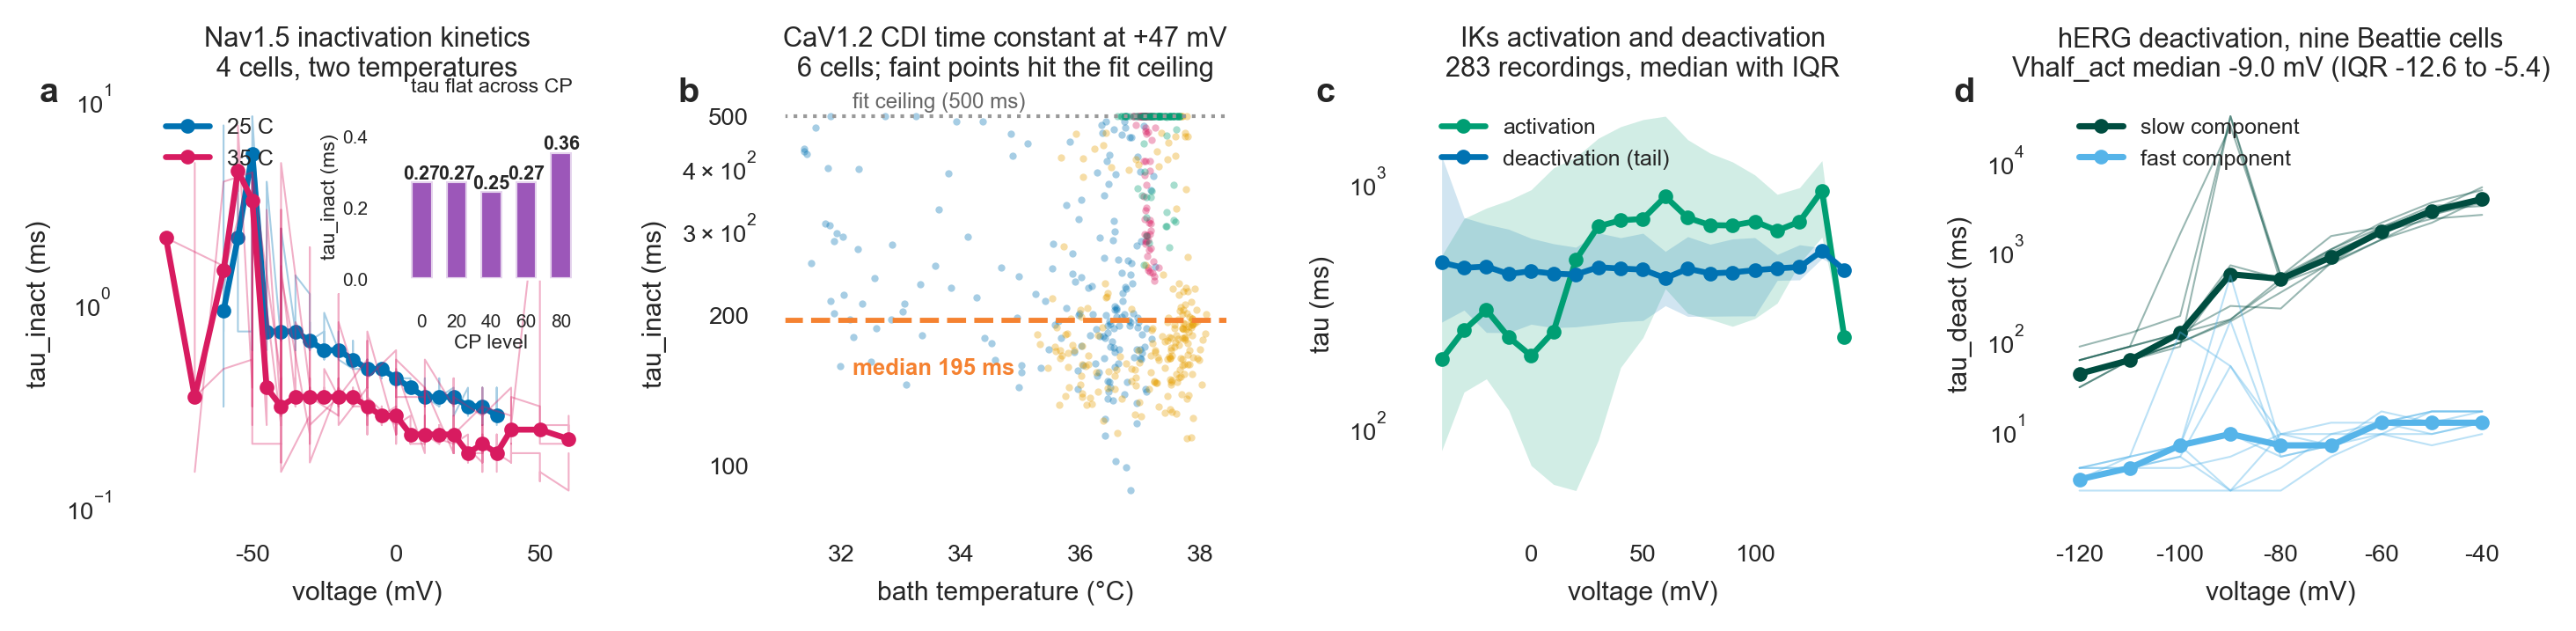
\includegraphics[width=\linewidth]{fig5_channel_cards.png}
\caption{\textbf{Channel cards from the unified table.} (a) Nav1.5 inactivation
time constant versus voltage at two temperatures (thin lines, individual cells;
heavy lines, medians). Inset: the same quantity across the five compound levels
of the study at 35\,$^\circ$C. (b) Ca\textsubscript{v}1.2 inactivation time
constant at +47\,mV against bath temperature, six cells; faint points are flagged
at the fit ceiling, and the dashed line is the median of quality-passed sweeps.
(c) I\textsubscript{Ks} activation and deactivation time constants, medians with
interquartile bands across 283 recordings. (d) hERG deactivation, two
exponential components, nine cells (thin) and medians (heavy).}
\label{fig:cards}
\end{figure}

\subsection{Measured tables forward-predict}

The point of a conserved quantity is that it can be carried into a model without
refitting. We assembled channel models in the form
$I = G\,m\,h\,(V - E_{\mathrm{rev}})$, with every voltage dependence a measured
table and the per-cell conductance $G$ the only free parameter, and we tested the
hardest available carry: replace the sealed hERG kinetics of the assembled model
by the Channelpedia population time-constant table, measured in a different
laboratory on an automated rig, and predict the manual-patch CiPA drug-screening
traces cell by cell. The population-table model passes the frozen acceptance
criteria in 67 of 68 cells (laboratory 3: 20/20; laboratory 4: 16/16; laboratory
5: 29/32; manual: 3/3), improving on the sealed-table model (65/68) while no cell
moves from pass to fail. The two rescued cells sit in laboratory 5, whose
recordings carry the largest voltage-clamp uncertainty of the panel, so the
population table adds information exactly where the single-cell tables are
weakest.

The assembly is compatible with the regulatory host end to end. Substituted into
the O'Hara--Rudy human ventricular model in place of the published hERG and
I\textsubscript{Ks} formulations, the measured tables preserve action-potential
morphology (APD90 difference 0.36\% at 1\,Hz steady state) and per-drug qNet
tracking through the dynamic-binding CiPA pipeline ($\rho=0.998$ against the
official arm on the 24 shared risk-labelled drugs). A measurement-table model
can therefore enter the existing scoring pipeline without changing its outputs
materially, while every one of its parameters is an auditable measurement rather
than a fitted constant.

\begin{figure}[htbp]
\centering
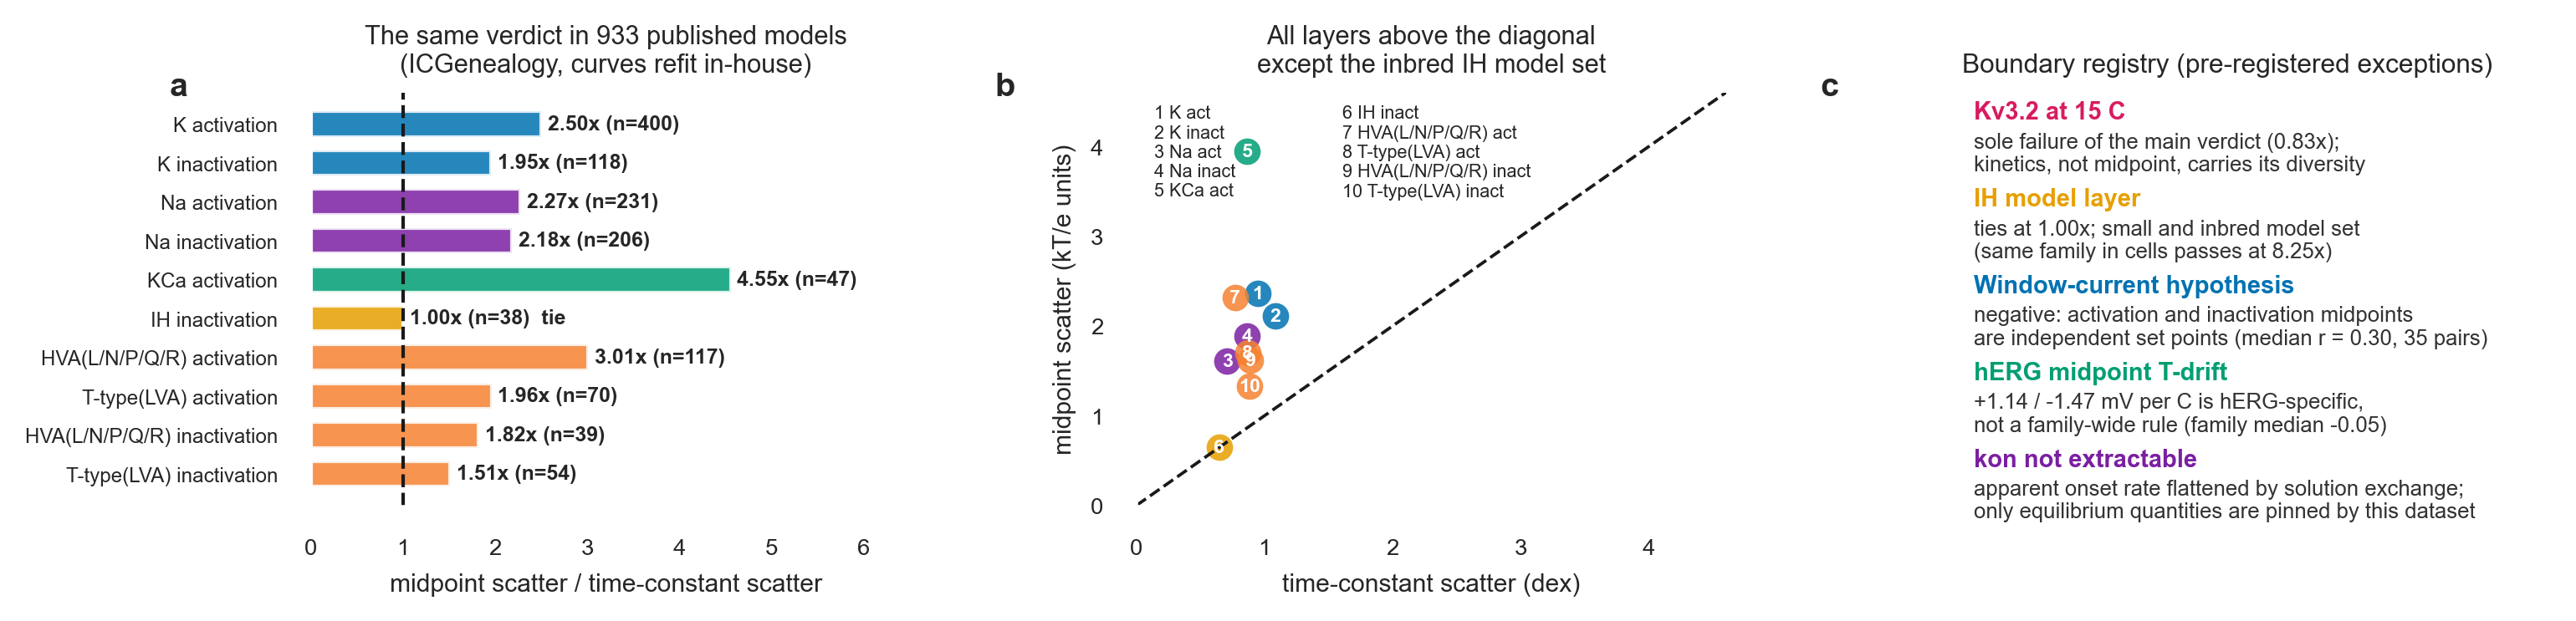
\includegraphics[width=\linewidth]{fig6_icg_boundary.png}
\caption{\textbf{The model literature and the boundary registry.} (a) The verdict
ratio for ten gating layers of 933 deduplicated published models (ICGenealogy),
curves refit in-house; the I\textsubscript{H} layer ties. (b) The two scatters
per layer; all layers sit above the diagonal except the inbred
I\textsubscript{H} set (numbered points keyed in panel). (c) The pre-registered
exceptions and negative results, carried with the paper rather than smoothed
over.}
\label{fig:icg}
\end{figure}

\section{Discussion}

A decade of identifiability work showed that the rate constants of channel models
cannot be recovered from voltage-clamp data. This paper maps the complementary
question, what the data do determine, at the scale the public record now allows.
The answer has two parts. Structurally, the data pin time and steady state while
leaving amplitude free (Eqs.~\eqref{eq:rescale}--\eqref{eq:factor}).
Empirically, the quantities the data pin are the quantities cells share. Across
seven corpora, one verdict rule finds time constants conserved and midpoints
cell-specific in nearly every group, and the same asymmetry reappears in
published models and across species. The two halves support each other: the
modal coordinates are measurable precisely because they are constrained, and they
are worth measuring because they are the stable content of the channel.

The biological reading is that a channel type is specified by its kinetics, while
each cell tunes where on the voltage axis those kinetics operate. Midpoints shift
with expression background, auxiliary subunits, phosphorylation and lipid state,
all of which vary between cells and preparations; kinetics are set by the
conformational free-energy landscape of the pore protein itself. The cross-species
layer makes the same point over evolutionary rather than cell-to-cell distance.

For modelling practice the recommendation is concrete. Spend parameters on
kinetic tables, which are conserved and therefore transferable, and fit midpoints
per cell, which are not. A model built this way needs one free conductance per
cell and predicts held-out protocols, cells and laboratories. For drug safety the
corollary is that the action of a drug on a channel is, to first order, a change
in occupancy tables rather than in kinetics, with a bounded kinetic correction of
at most about 20\% in the worst laboratory of a regulatory-scale dataset. Risk
scores built on IC$_{50}$ alone discard the state-dependence signatures visible
in the waveforms, which is where the residual risk information lives.

The boundaries are part of the result (Fig.~\ref{fig:icg}c). Kv3.2 at low
temperature stores its diversity in kinetics. The I\textsubscript{H} model layer
ties, and the inbred structure of that model set is the likely reason.
Activation and inactivation midpoints are independent set points, not a coupled
window. The apparent drug on-rate is not extractable from exchange-limited
recordings. Kir and K2P channels, whose currents are leak-like or
rectification-dominated rather than gated by S-shaped curves, do not enter the
verdict at all, and the Ca\textsubscript{v}1.2 arm rests on six cells. None of
these exceptions weakens the main statement, and all of them are where the next
corpora should look first.

Three limitations deserve emphasis. First, conservation is proven against
cell-to-cell scatter within a preparation, not against every possible biological
perturbation; disease remodelling, for example, may move kinetics as well as
midpoints, and the table makes that question directly testable. Second, the
verdict rule compares dimensionless scatters, and its threshold at one is a
convention; the conclusions rest on the size and unanimity of the effect, not on
the threshold. Third, the profile pipeline assumes the segment-local error model
of each extraction, and where that model is wrong the intervals are wrong with
it; the calibration panel (Fig.~\ref{fig:corpus}c) is the empirical check, and
it currently holds within a few percent of nominal.

The master table, the extraction code and the per-layer verdict tables are
public (Methods, Data availability). Every number in this paper can be
regenerated from the raw waveforms by the frozen pipeline, and every extracted
quantity carries its own uncertainty interval and quality flag, so the claims
here can be audited row by row.

\section{Methods}

\subsection{Data}

Seven public voltage-clamp corpora and three reference layers were used
(Table~\ref{tab:data}). (i) Channelpedia: automated patch-clamp recordings of
ion-channel cell lines (19,282 cells; 17,987 after quality control), covering
Kv, HCN, Kir, K2P and other families at 15, 25 and 35\,$^\circ$C, distributed as
NWB files and per-cell JSON. (ii) CiPA five-laboratory hERG: manual patch-clamp
recordings coordinated by HESI under the FDA Broad Agency Announcement, 28 drugs
under the standardised ICH S7B Q\&A 2.1 protocol with blinded replicate
arms~\cite{AlvarezBaron2025}; raw per-cell waveforms (62\,GB, sha256-verified)
at OSF osf.io/a6k5t; 1,875 cells passed trace-level quality control in our
reanalysis, of which 1,750 contribute deactivation time constants to the master
table. (iii) hERG five-temperature series~\cite{Lei2019b} (670 wells,
25--37\,$^\circ$C). (iv) Nine-cell manual hERG dataset~\cite{Beattie2018}
(figshare doi:10.6084/m9.figshare.4702546). (v) Nav1.5 whole-cell series at 25
and 35\,$^\circ$C under five compound levels~\cite{Lei2025} (figshare
doi:10.6084/m9.figshare.27193878). (vi) Ca\textsubscript{v}1.2 pharmacology
dataset with Ca$^{2+}$ and Ba$^{2+}$ carriers and continuous bath-temperature
readout~\cite{Ren2022} (OSF g3msb). (vii) I\textsubscript{Ks} activation
series~\cite{Fedida2024,Chan2023} (Zenodo 8226585). Reference layers: official
CiPA potency anchors for 29 drugs and seven channels; cross-species group
comparisons computed from layer (i); and gating curves of 933 deduplicated
published models from ICGenealogy, refit in-house.

\subsection{Extraction and profile-likelihood intervals}

Each protocol segment was reduced locally: mono- or bi-exponential fits to
activation, inactivation, deactivation and tail segments (component count fixed
per channel); Boltzmann fits to steady-state activation and availability; delays
by back-extrapolation to current onset, following published good-practice
guidelines~\cite{Montnach2021}. No objective function couples protocols
or parameters. Fit windows were set by protocol segment boundaries. Every
extracted quantity carries a per-row 95\% profile-likelihood interval obtained by
refitting the nuisance parameters on a grid over the target parameter and
applying the $F$-statistic threshold. Rows whose estimate reaches a fit boundary
are flagged \texttt{tau\_edge} and retained. The unified schema assigns source,
dataset, cell, channel, family, temperature, parameter, process, voltage, value,
interval, model, quality flag, method version, drug and blinding status to every
row.

\subsection{Conservation verdict}

For each channel-by-temperature group with at least 15 cells, the time-constant
scatter is the median over voltages of the across-cell standard deviation of
$\log_{10}\tau$, and the midpoint scatter is the across-cell standard deviation
of $V_{1/2}$ divided by the median Boltzmann slope $k$. Group-level true scatter
was estimated by hierarchical partial pooling with marginal likelihood, with
per-row standard errors taken from the profile intervals (asymmetric half-widths
averaged). The verdict ratio is midpoint scatter over time-constant scatter; a
ratio above one marks the time constant as the more conserved quantity. The same
rule was applied to the published-model layer after refitting each gating curve.

\subsection{Temperature analysis and forecast}

Pooled $Q_{10}$ values were estimated per channel, process and voltage from
cross-temperature pairs, and per process by median aggregation. The
zero-parameter forecast divides the 25\,$^\circ$C population table by the pooled
$Q_{10}$ and compares against the measured 35\,$^\circ$C population table at
matching channel, process and voltage.

\subsection{Drug reanalysis}

CiPA waveforms were segmented per cell into vehicle, drug-block and steady-state
windows without using the summary metadata (segmentation was validated against
the two directories that carry metadata). Tail deactivation time constants were
extracted per sweep with profile intervals; the per-cell ratio references the
steady-state window to the vehicle window of the same cell. Series-resistance
robustness, blinded-arm concordance, concentration monotonicity, onset-rate
flattening and the defect registry were computed as frozen audit stages on the
same extraction.

\subsection{Model assembly and host-model tests}

Channel models were assembled as $I = G\,m\,h\,(V-E_{\mathrm{rev}})$ with measured
tables and a per-cell conductance $G$ as the only free parameter. The
cross-laboratory test substitutes the Channelpedia population time-constant table
for the sealed hERG kinetics and scores prediction of CiPA screening traces under
the frozen acceptance criteria (67/68 with the population table, 65/68 with the
sealed table, no pass-to-fail flips). The O'Hara--Rudy host tests kept the
published Na\textsubscript{v}1.5 and Ca\textsubscript{v}1.2 formulations and
replaced $I_{\mathrm{Kr}}$ and $I_{\mathrm{Ks}}$ by the measured-table
implementations; APD90 was measured at 1\,Hz steady state and qNet tracking
followed the published dynamic-binding pipeline.

\subsection{Identifiability analysis}

The thirteen-parameter formulation, its calibration, and the Fisher matrix of
Eq.~\eqref{eq:fisher} are described in the Supplementary Information. Derivatives
were evaluated by central finite differences (step $10^{-3}$\,dex for log-scaled
parameters) on an independent simulation channel, with per-segment residual
variance as weights. Null directions were defined as eigenvalues below $10^{-3}$
of the largest.

\subsection{Statistics}

Group verdicts are reported as pass counts with median ratios; dispersion ratios
use hierarchical shrinkage as above; temperature scaling uses Arrhenius and
log-linear regression; correlations are Spearman. No $p$-value is reported for
comparisons that were not specified before the analysis. All statistics were
computed from the master table by the deposited scripts.

\section*{Data and code availability}

\begin{sloppypar}
All source datasets are public (Table~\ref{tab:data}). The master table, the
extraction and verdict code, the figure scripts and the per-layer verdict tables
are deposited at Zenodo (\url{https://doi.org/10.5281/zenodo.23042211}) and
mirrored at GitHub
(\url{https://github.com/lihuanlz/alpha-ion-channel-models}). The earlier
four-channel preprint is at Research Square
(\url{https://doi.org/10.21203/rs.3.rs-11218939/v1}).
\end{sloppypar}

\section*{Competing interests}

The author is employed by Shanghai Liangta Biotech Co., Ltd.

\begin{table}[htbp]
\centering
\caption{\textbf{Data inventory.} Seven experimental corpora were re-extracted
from raw waveforms by the unified profile-likelihood pipeline; three reference
layers are stored in the same schema. Row and cell counts refer to the master table.}
\label{tab:data}
\small
\begin{tabular}{p{3.4cm}p{5.2cm}rr}
\toprule
Corpus & Content & Rows & Cells \\
\midrule
Channelpedia & 74 channel types, automated patch, 15/25/35\,$^\circ$C & 276,039 & 17,987 \\
CiPA five-laboratory hERG & 28 drugs, blinded arms, manual patch & 192,055 & 1,750 \\
Lei 2019 five-temperature & hERG, 25--37\,$^\circ$C, automated & 10,203 & 670 \\
Beattie 2018 nine-cell & hERG, six protocols, manual & 207 & 9 \\
Nav1.5 (27193878) & two temperatures, five compound levels & 371 & 4 \\
Ca\textsubscript{v}1.2 (Ren 2022) & Ca$^{2+}$/Ba$^{2+}$, bath-temperature readout & 562 & 6 \\
I\textsubscript{Ks} (Fedida/Chan) & activation series & 8,147 & 283 \\
\midrule
Reference: CiPA anchors & official IC$_{50}$ and Hill, 29 drugs $\times$ 7 channels & 250 & \\
Reference: cross-species & 38 pairs, fold and midpoint differences & 76 & \\
Reference: ICGenealogy & 933 models refit, ten gating layers & 30 & \\
\bottomrule
\end{tabular}
\end{table}

\begin{table}[htbp]
\centering
\caption{\textbf{Headline verdicts.} Ratio of midpoint scatter to time-constant
scatter (shrunk estimates with profile-interval uncertainties); a ratio above one
marks the time constant as the more conserved quantity.}
\label{tab:verdicts}
\small
\begin{tabular}{llrll}
\toprule
Layer & Process & Groups & Pass & Median ratio \\
\midrule
Channelpedia Kv & activation & 64 & 63 (98.4\%) & 2.47 \\
Channelpedia Kv & deactivation & 48 & 43 (89.6\%) & 2.82 \\
Channelpedia Kv & inactivation & 35 & 28 (80.0\%) & 1.33 \\
Channelpedia Kv & recovery & 42 & 39 (92.9\%) & 2.15 \\
Channelpedia HCN & activation (reversed) & 5 & 5 (100\%) & 8.03 \\
ICGenealogy models & ten family-by-gate layers & 10 & 9 (90\%) & 2.07 \\
Cross-species pairs & two-fold window on $\tau$ & 38 & 38 (100\%) & \\
\bottomrule
\end{tabular}
\end{table}

\begin{thebibliography}{99}

\bibitem{Colatsky2016} Colatsky T, et al. The Comprehensive in Vitro
Proarrhythmia Assay (CiPA) initiative---update on progress. \emph{J Pharmacol
Toxicol Methods} 81:15--20 (2016). doi:10.1016/j.vascn.2016.06.002

\bibitem{Li2017} Li Z, et al. Improving the in silico assessment of
proarrhythmia risk by combining hERG (human ether-\`a-go-go-related gene)
channel--drug binding kinetics and multichannel pharmacology. \emph{Circ
Arrhythm Electrophysiol} 10:e004628 (2017). doi:10.1161/circep.116.004628

\bibitem{Dutta2017} Dutta S, Chang KC, Beattie KA, Sheng J, Tran PN, Wu WW,
Wu M, Strauss DG, Colatsky T, Li Z. Optimization of an in silico cardiac cell
model for proarrhythmia risk assessment. \emph{Front Physiol} 8:616 (2017).
doi:10.3389/fphys.2017.00616

\bibitem{OHara2011} O'Hara T, Vir\'ag L, Varr\'o A, Rudy Y. Simulation of the
undiseased human cardiac ventricular action potential: model formulation and
experimental validation. \emph{PLoS Comput Biol} 7:e1002061 (2011).
doi:10.1371/journal.pcbi.1002061

\bibitem{Clerx2016} Clerx M, Collins P, de Lange E, Volders PGA.
Myokit: a simple interface to cardiac cellular electrophysiology.
\emph{Prog Biophys Mol Biol} 120:100--114 (2016).
doi:10.1016/j.pbiomolbio.2015.12.008

\bibitem{Fink2009} Fink M, Noble D. Markov models for ion channels: versatility
versus identifiability and speed. \emph{Phil Trans R Soc A} 367:2161--2179
(2009). doi:10.1098/rsta.2008.0301

\bibitem{Beattie2018} Beattie KA, Hill AP, Bardenet R, Cui Y, Vandenberg JI,
Gavaghan DJ, de Boer TP, Mirams GR. Sinusoidal voltage protocols for rapid
characterisation of ion channel kinetics. \emph{J Physiol} 596:1813--1828
(2018). doi:10.1113/JP275733

\bibitem{Clerx2019} Clerx M, Robinson M, Lambert B, Lei CL, Ghosh S, Mirams GR,
Gavaghan DJ. Probabilistic inference on noisy time series (PINTS).
\emph{J Open Res Softw} 7:23 (2019). doi:10.5334/jors.252

\bibitem{AlvarezBaron2025} Alvarez Baron C, Zhao J, Yu H, Ren M, Thiebaud N,
Guo D, et al. Multi-laboratory comparisons of manual patch clamp hERG data
generated using standardized protocols and following ICH S7B Q\&A 2.1 best
practices. \emph{Sci Rep} 15:29995 (2025). doi:10.1038/s41598-025-15761-8.
Raw waveforms and summary tables: OSF osf.io/a6k5t.

\bibitem{Lei2019a} Lei CL, Clerx M, Gavaghan DJ, Polonchuk L, Mirams GR, Wang K.
Rapid characterization of hERG channel kinetics I: using an automated
high-throughput system. \emph{Biophys J} 117:2438--2454 (2019).
doi:10.1016/j.bpj.2019.07.029

\bibitem{Lei2019b} Lei CL, Clerx M, Beattie KA, Melgari D, Hancox JC,
Gavaghan DJ, Polonchuk L, Wang K, Mirams GR. Rapid characterization of hERG
channel kinetics II: temperature dependence. \emph{Biophys J} 117:2455--2470
(2019). doi:10.1016/j.bpj.2019.07.030

\bibitem{Lei2025} Lei CL, Clark AP, Clerx M, Wei S, Bloothooft M, de Boer TP,
Christini DJ, Krogh-Madsen T, Mirams GR. Resolving artifacts in voltage-clamp
experiments with computational modeling: an application to fast sodium current
recordings. \emph{Adv Sci} 12:e00691 (2025). doi:10.1002/advs.202500691

\bibitem{Ren2022} Ren M, et al. Experimental factors that impact
Ca\textsubscript{v}1.2 channel pharmacology---effects of recording temperature,
charge carrier, and quantification of drug effects on the step and ramp
currents elicited by the ``step-step-ramp'' voltage protocol. \emph{PLoS ONE}
17:e0276995 (2022). doi:10.1371/journal.pone.0276995

\bibitem{Fedida2024} Fedida D, Sastre D, Dou Y, Westhoff M, Eldstrom J.
Evaluating sequential and allosteric activation models in I\textsubscript{Ks}
channels with mutated voltage sensors. \emph{J Gen Physiol} 156(3):e202313465
(2024). doi:10.1085/jgp.202313465

\bibitem{Chan2023} Chan M, et al. A generic binding pocket for small-molecule
I\textsubscript{Ks} activators at the extracellular inter-subunit interface of
KCNQ1 and KCNE1 channel complexes. \emph{eLife} 12:RP87038 (2023).
doi:10.7554/eLife.87038

\bibitem{Vandenberg2006} Vandenberg JI, Varghese A, Lu Y, Bursill JA,
Mahaut-Smith MP, Huang C. Temperature dependence of human
ether-\`a-go-go-related gene K$^+$ currents. \emph{Am J Physiol Cell Physiol}
291:C165--C175 (2006). doi:10.1152/ajpcell.00596.2005

\bibitem{Li2016} Li Z, Dutta S, Sheng J, Tran PN, Wu W, Colatsky T. A
temperature-dependent in silico model of the human ether-\`a-go-go-related
(hERG) gene channel. \emph{J Pharmacol Toxicol Methods} 81:233--239 (2016).
doi:10.1016/j.vascn.2016.05.005

\bibitem{Montnach2021} Montnach J, Lorenzini M, Lesage A, Simon I, Nicolas S,
Moreau E, Marionneau C, Bar\'o I, De Waard M, Loussouarn G. Computer modeling of
whole-cell voltage-clamp analyses to delineate guidelines for good practice of
manual and automated patch-clamp. \emph{Sci Rep} 11:3282 (2021).
doi:10.1038/s41598-021-82077-8

\end{thebibliography}

\end{document}
